\documentclass[a4paper, 12pt]{article}

%%% Работа с русским языком
\usepackage{cmap}					% поиск в PDF
\usepackage{mathtext} 				% русские буквы в формулах
\usepackage[T2A]{fontenc}			% кодировка
\usepackage[utf8]{inputenc}			% кодировка исходного текста
\usepackage[russian]{babel}	% локализация и переносы

%%% Дополнительная работа с математикой
\usepackage{amsmath,amsfonts,amssymb,amsthm,mathtools} % AMS
\usepackage{icomma} % "Умная" запятая: $0,2$ --- число, $0, 2$ --- перечисление

%% Номера формул
%\mathtoolsset{showonlyrefs=true} % Показывать номера только у тех формул, на которые есть \eqref{} в тексте.

%% Шрифты
\usepackage{euscript}	 % Шрифт Евклид
\usepackage{mathrsfs} % Красивый матшрифт

%% Поля
\usepackage[left=2cm,right=2cm,top=2cm,bottom=2cm,bindingoffset=0cm]{geometry}

%% Русские списки
\usepackage{enumitem}
\makeatletter
\AddEnumerateCounter{\asbuk}{\russian@alph}{щ}
\makeatother

%%% Работа с картинками
\usepackage{graphicx}  % Для вставки рисунков
\graphicspath{{images/}{images2/}}  % папки с картинками
\setlength\fboxsep{3pt} % Отступ рамки \fbox{} от рисунка
\setlength\fboxrule{1pt} % Толщина линий рамки \fbox{}
\usepackage{wrapfig} % Обтекание рисунков и таблиц текстом

%%% Работа с таблицами
\usepackage{array,tabularx,tabulary,booktabs} % Дополнительная работа с таблицами
\usepackage{longtable}  % Длинные таблицы
\usepackage{multirow} % Слияние строк в таблице

%% Красная строка
\setlength{\parindent}{2em}

%% Интервалы
\linespread{1}
\usepackage{multirow}

%% TikZ
\usepackage{tikz}
\usetikzlibrary{graphs,graphs.standard}

%% Верхний колонтитул
\usepackage{fancyhdr}
\pagestyle{fancy}

%% Перенос знаков в формулах (по Львовскому)
\newcommand*{\hm}[1]{#1\nobreak\discretionary{}
	{\hbox{$\mathsurround=0pt #1$}}{}}

%% Мои дополнения
\usepackage{float} %Добавляет возможность работы с командой [H] которая улучшает расположение на странице
\usepackage{gensymb} %Красивые градусы
\usepackage{graphicx}               % Импорт изображений
\usepackage{caption} % Пакет для подписей к рисункам, в частности, для работы caption*

% подключаем hyperref (для ссылок внутри  pdf)
\usepackage[unicode, pdftex]{hyperref}

%%% Теоремы
\theoremstyle{plain}                    % Это стиль по умолчанию, его можно не переопределять.
\renewcommand\qedsymbol{$\blacksquare$} % переопределение символа завершения доказательства

\newtheorem{theorem}{Теорема}[section] % Теорема (счетчик по секиям)
\newtheorem{proposition}{Утверждение}[section] % Утверждение (счетчик по секиям)
\newtheorem{definition}{Определение}[section] % Определение (счетчик по секиям)
\newtheorem{corollary}{Следствие}[theorem] % Следстиве (счетчик по теоремам)
\newtheorem{problem}{Задача}[section] % Задача (счетчик по секиям)
\newtheorem*{remark}{Примечание} % Примечание (можно переопределить, как Замечание)
\newtheorem{lemma}{Лемма}[section] % Лемма (счетчик по секиям)

\begin{document}
    \newcommand{\HRule}{\rule{\linewidth}{0.7mm}} % Defines a new command for the horizontal lines, change thickness here
	
	\begin{center}
		\large\textbf{Московский Физико-Технический Институт}\\ % Name of your university/college
		\large\textbf{(государственный университет)}
	
		\vfill
		
		\Large Лабораторная работа по курсу общей физики № *labnum*\\[0.5cm] % Preambule of your document title
		
		
		\HRule
		\\[0.4cm]
		{ \huge \bfseries *name of your labwork*}% Title of your document
		\\[0.4cm] 
		\HRule
		\\[0.5cm]
		
		\ \\
	\textbf{\large Автор:} \\	
	\large *your name* *groupname*\\ % Your name and something more, your group num for example
		\vfill
		\hspace*{-0.8 cm}
\includegraphics[width=100 pt]{frkt_logo}\\ % logo of your  company/university/college
		\large Долгопрудный, 2021 % location and year
	\end{center}

\newpage
\setcounter{page}{2}
\fancyfoot[c]{\thepage}
\fancyhead[L] {Работа № *labnum*} % some information in page header
\fancyhead[R]{}

    \section{Расчетные формулы}

    \begin{enumerate}

		\item Температура электронов:
        \begin{equation} \label{electron Temperature}
            T_e = \frac{1}{2k_\text{Б}}\frac{eI_i}{\frac{dI}{dU}|_{U = 0}}
        \end{equation}	
        \item Электронный ток насыщения [СИ]:
        \begin{equation} \label{saturation current}
            I_i \simeq 0.4 n_e e S \sqrt{\frac{2k_\text{Б}T_e}{m_i}}
        \end{equation}	
        \item Плазменная(ленгмюровская) частота [СГС]:
        \begin{equation} \label{omega_p}
            \omega_p = \sqrt{\frac{4\pi n_e e^2}{m_e}} \approx 5.6 \cdot 10^4 \sqrt{n_e}
        \end{equation}
        \item Электронная поляризационная длина [СГС]:
        \begin{equation} \label{r_{De}}
            r_{De} = \sqrt{\frac{k_\text{Б}T_e}{4\pi n_e e^2}}      
        \end{equation}
        \item Ионная поляризационная длина [СГС]:
        \begin{equation} \label{r_{Di}}
            r_{Di} = \sqrt{\frac{k_\text{Б}T_i}{4\pi n_i e^2}}
        \end{equation}
        \item Дебаевский радиус [СГС] (в предположениии $T_i \ll T_e$):
        \begin{equation} \label{r_D}
            r_D = (r_{De}^{-2} + r_{Di}^{-2})^{-1/2} = \sqrt{\frac{k_{\text{Б}}}{2 \pi n_e e^2} \frac{T_e T_i}{T_e + T_i}} \approx \sqrt{\frac{k_\text{Б}T_i}{4\pi n_i e^2}}
        \end{equation}
        \item Среднее число ионов в дебаевской сфере:
        \begin{equation} \label{N_i}
            N_i = \frac{4}{3} \pi r_D^3 n_i
        \end{equation}
        \item Степень ионизации плазмы ($P$ -- давление в трубке):
        \begin{equation} \label{alpha}
            \alpha = \frac{k_{\text{Б}} n_i T_i}{P}
        \end{equation}

	\end{enumerate}

    \section{Обработка эксперементальных данных}

    Запишем параметры установки
    \begin{center}
        Диаметр зонда $d = 0.2$ мм \\
        Длина зонда $l = 5.2$ мм \\
        Длина трубки $L \approx 35.5$ мм \\
    \end{center}

    Эксперементально установленное напряжение зажигания заряда $U_{\text{заж}} \approx 1.54$ кВ.

    Снимем вольт-амперную характеристику разряда.

    \begin{figure}
        \centering
        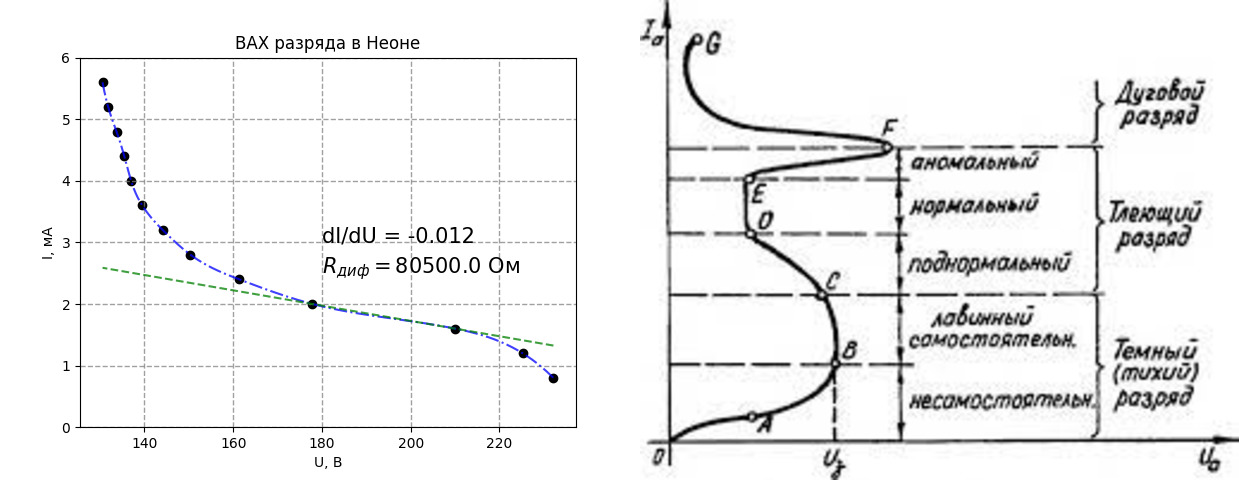
\includegraphics[width = \textwidth]{merged.jpg}
        \caption{Вольт-амперная характеристика разряда}
        \label{diagram}
    \end{figure}

    Сравнив имзеренный участок с \hyperref[diagram]{графиком}, приходим к выводу, что измеренный участок
    соответсвует участку $DC$ диаграммы. По наклону кривой определим максимальное
    дифференциальное сопротивление разряда.

    \begin{center}
        \fbox{$R_{\text{диф}} = 8.05 \cdot 10^4$ Ом}
    \end{center}

    Снимем зондовые характеристики при $I_p = 4.8$ мА, $I_p = 3$ мА, $I_p = 1.5$ мА.

    \begin{figure}
        \centering
        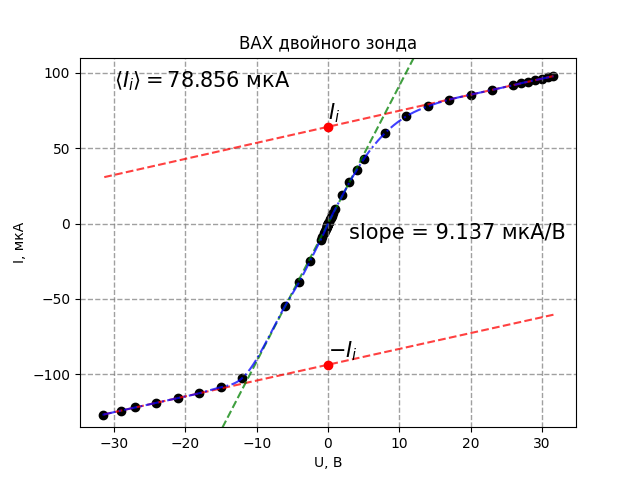
\includegraphics[width = 0.8\textwidth]{VAC2.png}
        \caption{$I_p = 4.8$ мА}
    \end{figure}

    \begin{figure}
        \centering
        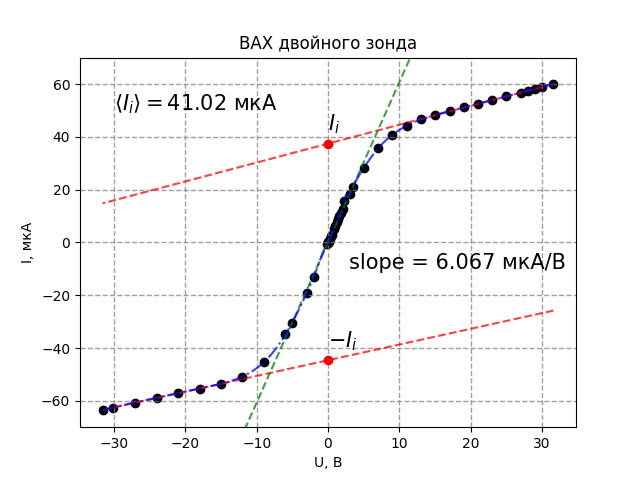
\includegraphics[width = 0.8\textwidth]{VAC3.png}
        \caption{$I_p = 3$ мА}
    \end{figure}

    \begin{figure}
        \centering
        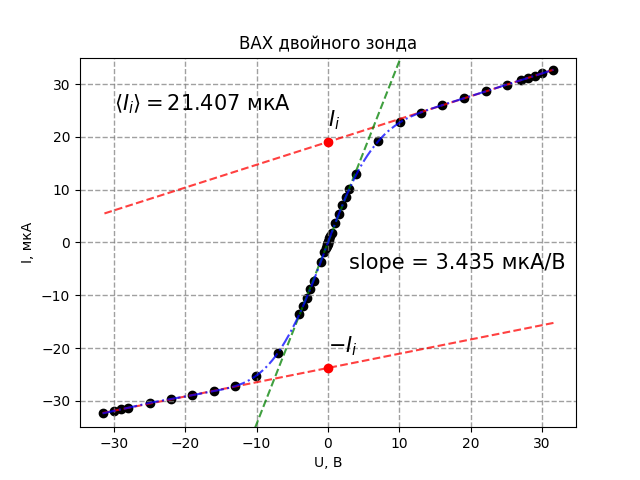
\includegraphics[width = 0.8\textwidth]{VAC4.png}
        \caption{$I_p = 1.5$ мА}
    \end{figure}

    \begin{figure}
        \centering
        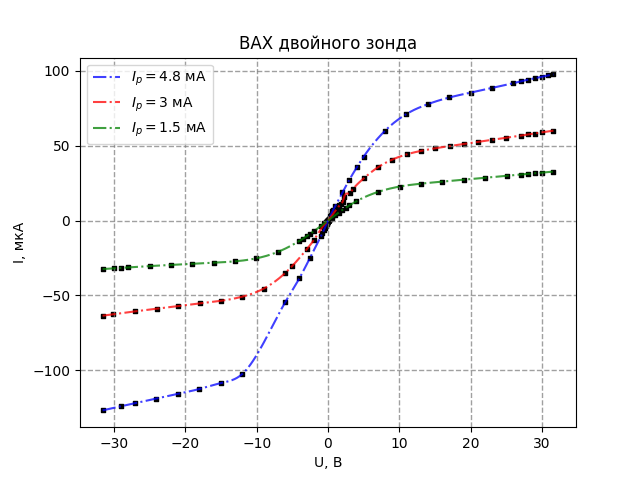
\includegraphics[width = 0.8\textwidth]{all_VAC.png}
    \end{figure}

    Для расчета температуры электронов $T_e$, концентрации электронов и ионов
    $n_e = n_i$ а так же плазменной частоты $\omega_p$ воспользуемся формулами 
    \eqref{electron Temperature} \eqref{saturation current} \eqref{omega_p}. 
    (Масса иона неона $m_i = 22 \cdot 1.66 \cdot 10^{-27}$ кг, заряд электрона в СГС $e = -4.8 \cdot 10^{-10}$ ед. зар.).

    \begin{table}[h!]
    \centering
    \begin{tabular}{|c|c|c|c|c|c|}
    \hline
    $I_i$, мкА & $dI/dU$, мкА/В & $T_e$, K  & $T_e$, эВ  & $n_e \cdot 10^{10}, ~ \text{см}^{-3}$ & $\omega_p \cdot 10^10$, рад/с \\ \hline
    78,856     & 9,137          & 50031,33  & 4,31       & 6,13                & 1,39                          \\ \hline
    41,02      & 6,067          & 39195,17  & 3,377      & 3,6                 & 1,06                          \\ \hline
    21,407     & 3,435          & 36127,67  & 3,11       & 1,96                & 0,79                          \\ \hline
    \end{tabular}
\end{table}

    Для расчета электронной поляризационной длинны $r_{De}$, радиуса экранирования $r_D$, среднего числа ионов в
    дебаевском радиусе $N_i$ и степени ионизации плазмы $\alpha$ воспользуемся формулами \eqref{r_{De}}, \eqref{r_D}, \eqref{N_i}, \eqref{alpha}.
    (Давление в трубке $P = 2$ торр).

    \begin{table}[h!]
    \centering
    \begin{tabular}{|c|c|c|c|c|}
    \hline
    $I_p$, мА & $r_{De} \cdot 10^{-1}$, см & $r_D \cdot 10^{-4}$, см & $N_e$ & $\alpha \cdot 10^{-7}$ \\ \hline
    5         & 6,23                       & 4,83                    & 29    & 9,52                   \\ \hline
    3         & 7,18                       & 6,3                     & 38    & 5,59                   \\ \hline
    1.5       & 9,38                       & 8,54                    & 51    & 3,04                   \\ \hline
    \end{tabular}
\end{table}

    Построим графики $T_e(I_p)$ и $n_e(I_p)$.

    \begin{figure}
        \centering
        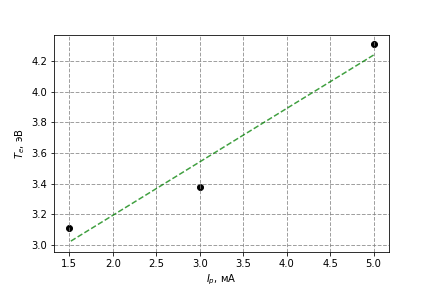
\includegraphics[width = 0.8\textwidth]{Te(Ip).png}
        \caption{График зависимости температуры электронов от тока заряда}
    \end{figure}

    \begin{figure}
        \centering
        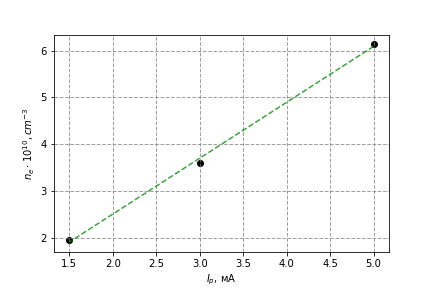
\includegraphics[width = 0.8\textwidth]{ne(Ip).png}
        \caption{График зависимости концентрации электронов от тока заряда}
    \end{figure}

    \textbf{Вывод:} как можно видеть из графиков, зависимости $T_e(I_p)$ и $n_e(I_p)$ практически линейный. 
    По результатам эксперемента можно считать, что $N_D \gg 1$, поэтому плазму в данном эксперементе можно считать идеальной.
    Кроме того, линейные размеры плазмы намного привосходят величину $r_{De}$,
    поэтому плазму можно считать квазинейтральной.

    \section{Таблицы эксперементальных данных}

    \begin{table}[h!]
    \centering
    \begin{tabular}{|c|c|}
        \hline
        $I$, мА & $U$, В   \\ \hline
        60      & 246,89   \\ \hline
        120     & 232,19   \\ \hline
        180     & 225,26   \\ \hline
        240     & 210,07   \\ \hline
        300     & 177,87   \\ \hline
        360     & 161,35   \\ \hline
        420     & 150,36   \\ \hline
        480     & 144,13   \\ \hline
        540     & 139,51   \\ \hline
        600     & 136,99   \\ \hline
        660     & 135,45   \\ \hline
        720     & 133,70   \\ \hline
        780     & 131,81   \\ \hline
        840     & 130,55   \\ \hline
    \end{tabular}
    \caption{ВАХ разряда в неоне}
    \label{VAC1}
\end{table}
    \begin{table}[h!]
    \centering
    \begin{tabular}{|c|c|c|c|}
        \hline
        $I$, мкА & $U$, В & $I$, мкА & $U$, В    \\ \hline
        123,34   & 31,61  & 2,17     & -0,008    \\ \hline
        122,77   & 30,9   & 2,11     & -0,015    \\ \hline
        121,79   & 29,97  & 2,07     & -0,019    \\ \hline
        120,86   & 29,08  & 1,96     & -0,027    \\ \hline
        119,82   & 28,07  & 1,65     & -0,05     \\ \hline
        118,77   & 27,02  & 1,23     & -0,086    \\ \hline
        117,5    & 25,99  & 0,8      & -0,119    \\ \hline
        114,37   & 23,04  & 0,43     & -0,154    \\ \hline
        111,22   & 20,03  & -0,18    & -0,208    \\ \hline
        107,95   & 17,03  & -1,21    & -0,302    \\ \hline
        103,54   & 14,04  & -2,81    & -0,45     \\ \hline
        96,88    & 11     & -4,38    & -0,6      \\ \hline
        85,83    & 8,02   & -6,43    & -0,8      \\ \hline
        68,47    & 5,01   & -8,42    & -1        \\ \hline
        61,25    & 4,03   & -22,63   & -2,509    \\ \hline
        53,09    & 3,01   & -36,27   & -4        \\ \hline
        44,62    & 2,03   & -52,54   & -6,02     \\ \hline
        35,33    & 1,01   & -70,49   & -9,02     \\ \hline
        32,72    & 0,72   & -100,41  & -12,053   \\ \hline
        31,86    & 0,63   & -106,36  & -15,03    \\ \hline
        30,75    & 0,51   & -110,39  & -18,11    \\ \hline
        29,54    & 0,39   & -113,52  & -21,05    \\ \hline
        28,62    & 0,3    & -116,67  & -24,08    \\ \hline
        27,1     & 0,145  & -119,74  & -27,02    \\ \hline
        26,36    & 0,069  & -121,86  & -29,06    \\ \hline
        25,76    & 0,007  & -124,59  & -31,61    \\ \hline
    \end{tabular}
    \caption{ВАХ двойного зонда при $I = 4.8$ мА}
    \label{VAC2}
\end{table}
    \begin{table}[h!]
    \centering
    \begin{tabular}{|c|c|c|c|}
    \hline
    $I$, мкА & $U$, В & $I$, мкА & $U$, В    \\ \hline
    72,77    & 31,61  & 19,02    & 0,995     \\ \hline
    71,64    & 30,04  & 17,77    & 0,8       \\ \hline
    70,84    & 28,96  & 15,59    & 0,5       \\ \hline
    70,21    & 28,08  & 15,08    & 0,4       \\ \hline
    69,44    & 27,01  & 14,13    & 0,246     \\ \hline
    68,04    & 25,02  & 13,02    & 0,1       \\ \hline
    66,6     & 22,99  & 12,73    & 0,045     \\ \hline
    65,23    & 21,03  & 8,23     & -0,019    \\ \hline
    63,88    & 19,08  & 8,28     & -0,035    \\ \hline
    62,48    & 17,07  & 8,03     & -0,055    \\ \hline
    60,93    & 14,98  & 7,66     & -0,104    \\ \hline
    59,29    & 13,082 & -4,97    & -2,013    \\ \hline
    56,9     & 11,02  & -11,07   & -3        \\ \hline
    53,31    & 8,95   & -22,12   & -5,02     \\ \hline
    48,43    & 7,05   & -26,64   & -5,97     \\ \hline
    40,98    & 5,03   & -37,17   & -9        \\ \hline
    33,85    & 3,52   & -42,59   & -12,013   \\ \hline
    31,13    & 3,02   & -45,37   & -15,026   \\ \hline
    28,24    & 2,25   & -47,15   & -17,98    \\ \hline
    25,44    & 2,07   & -48,89   & -21,04    \\ \hline
    23,93    & 1,8    & -50,61   & -23,99    \\ \hline
    22,78    & 1,6    & -52,42   & -27,085   \\ \hline
    21,57    & 1,4    & -54,34   & -30,13    \\ \hline
    20,34    & 1,2    & -55,3    & -31,61    \\ \hline
    \end{tabular}
    \caption{ВАХ двойного зонда при $I = $}
    \label{VAC3}
\end{table}
    \begin{table}[h!]
    \centering
    \begin{tabular}{|c|c|c|c|}
    \hline
    $I$, мкА & $U$, В   & $I$, мкА & $U$, В    \\ \hline
    39,29    & 31,6     & 5,92     & -0,02     \\ \hline
    38,63    & 30,03    & 5,77     & -0,05     \\ \hline
    38,18    & 29       & 5,63     & -0,1      \\ \hline
    37,74    & 28,01    & 5,26     & -0,2      \\ \hline
    37,32    & 27,04    & 4,89     & -0,29     \\ \hline
    36,46    & 25,06    & 4,14     & -0,499    \\ \hline
    35,19    & 22,08    & 2,31     & -1,01     \\ \hline
    33,88    & 19       & -1,22    & -2,01     \\ \hline
    32,61    & 16,045   & -2,89    & -2,5      \\ \hline
    31,2     & 12,98    & -4,55    & -3,01     \\ \hline
    29,32    & 10,07    & -6,1     & -3,5      \\ \hline
    25,79    & 7,06     & -7,58    & -4        \\ \hline
    19,51    & 3,99     & -14,89   & -7,008    \\ \hline
    16,75    & 3,006    & -19,21   & -10,025   \\ \hline
    15,24    & 2,5      & -21,22   & -13,004   \\ \hline
    13,65    & 2        & -22,17   & -16,02    \\ \hline
    11,89    & 1,506    & -22,95   & -19,06    \\ \hline
    10,21    & 1,002    & -23,68   & -22       \\ \hline
    8,45     & 0,504    & -24,4    & -25,01    \\ \hline
    7,73     & 0,3      & -25,34   & -28,06    \\ \hline
    7,37     & 0,2      & -25,62   & -29,04    \\ \hline
    6,97     & 0,098    & -25,92   & -30,04    \\ \hline
    6,6      & 0,005    & -26,39   & -31,6     \\ \hline
    6        & -0,0086  &          &           \\ \hline
    \end{tabular}
    \caption{ВАХ двойного зонда при $I = $}
    \label{VAC4}
\end{table}

\end{document}